\documentclass[
  shownotes,
  xcolor={svgnames},
  hyperref={colorlinks,citecolor=DarkBlue,linkcolor=DarkRed,urlcolor=DarkBlue}
  , aspectratio=169]{beamer}
\usepackage{animate}
\usepackage{amsmath}
\usepackage{amsfonts}
\usepackage{amssymb}
\usepackage{pifont}
\usepackage{mathpazo}
%\usepackage{xcolor}
\usepackage{multimedia}
\usepackage{fancybox}
\usepackage[para]{threeparttable}
\usepackage{multirow}
\setcounter{MaxMatrixCols}{30}
\usepackage{subcaption}
\usepackage{graphicx}
\usepackage{lscape}
\usepackage[compatibility=false,font=small]{caption}
\usepackage{booktabs}
\usepackage{ragged2e}
\usepackage{chronosys}
\usepackage{appendixnumberbeamer}
\usepackage{animate}
\setbeamertemplate{caption}[numbered]
\usepackage{color}
%\usepackage{times}
\usepackage{tikz}
\usepackage{comment} %to comment
%% BibTeX settings
\usepackage{natbib}
\bibliographystyle{apalike}
\bibpunct{(}{)}{,}{a}{,}{,}
\setbeamertemplate{bibliography item}{[\theenumiv]}

% Defines columns for bespoke tables
\usepackage{array}
\newcolumntype{L}[1]{>{\raggedright\let\newline\\\arraybackslash\hspace{0pt}}m{#1}}
\newcolumntype{C}[1]{>{\centering\let\newline\\\arraybackslash\hspace{0pt}}m{#1}}
\newcolumntype{R}[1]{>{\raggedleft\let\newline\\\arraybackslash\hspace{0pt}}m{#1}}


\usepackage{xfrac}


\usepackage{multicol}
\setlength{\columnsep}{0.5cm}

% Theme and colors
\usetheme{Boadilla}

% I use steel blue and a custom color palette. This defines it.
\definecolor{andesred}{HTML}{af2433}

% Other options
\providecommand{\U}[1]{\protect\rule{.1in}{.1in}}
\usefonttheme{serif}
\setbeamertemplate{itemize items}[default]
\setbeamertemplate{enumerate items}[square]
\setbeamertemplate{section in toc}[circle]

\makeatletter

\definecolor{mybackground}{HTML}{82CAFA}
\definecolor{myforeground}{HTML}{0000A0}

\setbeamercolor{normal text}{fg=black,bg=white}
\setbeamercolor{alerted text}{fg=red}
\setbeamercolor{example text}{fg=black}

\setbeamercolor{background canvas}{fg=myforeground, bg=white}
\setbeamercolor{background}{fg=myforeground, bg=mybackground}

\setbeamercolor{palette primary}{fg=black, bg=gray!30!white}
\setbeamercolor{palette secondary}{fg=black, bg=gray!20!white}
\setbeamercolor{palette tertiary}{fg=white, bg=andesred}

\setbeamercolor{frametitle}{fg=andesred}
\setbeamercolor{title}{fg=andesred}
\setbeamercolor{block title}{fg=andesred}
\setbeamercolor{itemize item}{fg=andesred}
\setbeamercolor{itemize subitem}{fg=andesred}
\setbeamercolor{itemize subsubitem}{fg=andesred}
\setbeamercolor{enumerate item}{fg=andesred}
\setbeamercolor{item projected}{bg=gray!30!white,fg=andesred}
\setbeamercolor{enumerate subitem}{fg=andesred}
\setbeamercolor{section number projected}{bg=gray!30!white,fg=andesred}
\setbeamercolor{section in toc}{fg=andesred}
\setbeamercolor{caption name}{fg=andesred}
\setbeamercolor{button}{bg=gray!30!white,fg=andesred}


\usepackage{fancyvrb}
\newcommand{\VerbBar}{|}
\newcommand{\VERB}{\Verb[commandchars=\\\{\}]}
\DefineVerbatimEnvironment{Highlighting}{Verbatim}{commandchars=\\\{\}}
% Add ',fontsize=\small' for more characters per line
\usepackage{framed}
\definecolor{shadecolor}{RGB}{248,248,248}
\newenvironment{Shaded}{\begin{snugshade}}{\end{snugshade}}
\newcommand{\AlertTok}[1]{\textcolor[rgb]{0.94,0.16,0.16}{#1}}
\newcommand{\AnnotationTok}[1]{\textcolor[rgb]{0.56,0.35,0.01}{\textbf{\textit{#1}}}}
\newcommand{\AttributeTok}[1]{\textcolor[rgb]{0.77,0.63,0.00}{#1}}
\newcommand{\BaseNTok}[1]{\textcolor[rgb]{0.00,0.00,0.81}{#1}}
\newcommand{\BuiltInTok}[1]{#1}
\newcommand{\CharTok}[1]{\textcolor[rgb]{0.31,0.60,0.02}{#1}}
\newcommand{\CommentTok}[1]{\textcolor[rgb]{0.56,0.35,0.01}{\textit{#1}}}
\newcommand{\CommentVarTok}[1]{\textcolor[rgb]{0.56,0.35,0.01}{\textbf{\textit{#1}}}}
\newcommand{\ConstantTok}[1]{\textcolor[rgb]{0.00,0.00,0.00}{#1}}
\newcommand{\ControlFlowTok}[1]{\textcolor[rgb]{0.13,0.29,0.53}{\textbf{#1}}}
\newcommand{\DataTypeTok}[1]{\textcolor[rgb]{0.13,0.29,0.53}{#1}}
\newcommand{\DecValTok}[1]{\textcolor[rgb]{0.00,0.00,0.81}{#1}}
\newcommand{\DocumentationTok}[1]{\textcolor[rgb]{0.56,0.35,0.01}{\textbf{\textit{#1}}}}
\newcommand{\ErrorTok}[1]{\textcolor[rgb]{0.64,0.00,0.00}{\textbf{#1}}}
\newcommand{\ExtensionTok}[1]{#1}
\newcommand{\FloatTok}[1]{\textcolor[rgb]{0.00,0.00,0.81}{#1}}
\newcommand{\FunctionTok}[1]{\textcolor[rgb]{0.00,0.00,0.00}{#1}}
\newcommand{\ImportTok}[1]{#1}
\newcommand{\InformationTok}[1]{\textcolor[rgb]{0.56,0.35,0.01}{\textbf{\textit{#1}}}}
\newcommand{\KeywordTok}[1]{\textcolor[rgb]{0.13,0.29,0.53}{\textbf{#1}}}
\newcommand{\NormalTok}[1]{#1}
\newcommand{\OperatorTok}[1]{\textcolor[rgb]{0.81,0.36,0.00}{\textbf{#1}}}
\newcommand{\OtherTok}[1]{\textcolor[rgb]{0.56,0.35,0.01}{#1}}
\newcommand{\PreprocessorTok}[1]{\textcolor[rgb]{0.56,0.35,0.01}{\textit{#1}}}
\newcommand{\RegionMarkerTok}[1]{#1}
\newcommand{\SpecialCharTok}[1]{\textcolor[rgb]{0.00,0.00,0.00}{#1}}
\newcommand{\SpecialStringTok}[1]{\textcolor[rgb]{0.31,0.60,0.02}{#1}}
\newcommand{\StringTok}[1]{\textcolor[rgb]{0.31,0.60,0.02}{#1}}
\newcommand{\VariableTok}[1]{\textcolor[rgb]{0.00,0.00,0.00}{#1}}
\newcommand{\VerbatimStringTok}[1]{\textcolor[rgb]{0.31,0.60,0.02}{#1}}
\newcommand{\WarningTok}[1]{\textcolor[rgb]{0.56,0.35,0.01}{\textbf{\textit{#1}}}}
\usepackage{graphicx}
\makeatletter

\usepackage{tikz}
% Tikz settings optimized for causal graphs.
\usetikzlibrary{shapes,decorations,arrows,calc,arrows.meta,fit,positioning}
\tikzset{
    -Latex,auto,node distance =1 cm and 1 cm,semithick,
    state/.style ={ellipse, draw, minimum width = 0.7 cm},
    point/.style = {circle, draw, inner sep=0.04cm,fill,node contents={}},
    bidirected/.style={Latex-Latex,dashed},
    el/.style = {inner sep=2pt, align=left, sloped}
}


\makeatother






%%%%%%%%%%%%%%% BEGINS DOCUMENT %%%%%%%%%%%%%%%%%%

\begin{document}

\title[Lecture 10]{Lecture 10: Bayesian Estimation \& Empirical Bayes}
\subtitle{Big Data and Machine Learning for Applied Economics \\ Econ 4676}
\date{\today}

\author[Sarmiento-Barbieri]{Ignacio Sarmiento-Barbieri}
\institute[Uniandes]{Universidad de los Andes}


\begin{frame}[noframenumbering]
\maketitle
\end{frame}

%%%%%%%%%%%%%%%%%%%%%%%%%%%%%%%%%%%


%----------------------------------------------------------------------% 

\begin{frame}
\frametitle{Agenda}

\tableofcontents


\end{frame}

%----------------------------------------------------------------------% 
\section{Recap Bayes Theorem}
%----------------------------------------------------------------------%
\begin{frame}[fragile]
\frametitle{Bayes Theorem}


\bigskip
\begin{align}
\pi (\theta|X)=\frac{f(X|\theta)p(\theta)}{m(X)}
\end{align}

\bigskip
with $m(X)$ is the marginal distribution of $X$, i.e.

\begin{align}
m(X)=\int f(X|\theta)p(\theta)d\theta
\end{align}

It is important to note that Bayes' theorem  does not tell us what our beliefs should be, it tells us how they should change after seeing new information.
\end{frame}


%----------------------------------------------------------------------%
\section{Empirical Bayes}
%----------------------------------------------------------------------%
\subsection{Motivation}
%----------------------------------------------------------------------%
\begin{frame}[fragile]
\frametitle{Motivation}


\begin{itemize}
  \small
\item The constraints of slow mechanical computation molded classical statistics into a mathematically ingenious theory of sharply delimited scope. 
\medskip
\item After WW2, computers  allowed a more expansive and useful statistical methodology.
\medskip
\item However, Some revolutions start slowly. The journals of the 1950s continued to emphasize classical themes
\medskip
\item Change came gradually, but by the 1990s a new statistical technology, computer enabled, was firmly in place. 
\medskip
\item Empirical Bayes methodology, has been a particularly slow developer despite an early start in the 1940s. 
\medskip
\item The roadblock here was not so much the computational demands of the theory as a lack of appropriate data sets. 

\end{itemize}
\end{frame}


%----------------------------------------------------------------------%
\begin{frame}[fragile]
\frametitle{Motivation}

\begin{itemize}
\item In Economics this revolution is starting to catch up, fueled by Big Data
\end{itemize}

\begin{figure}[H] \centering
  \centering
  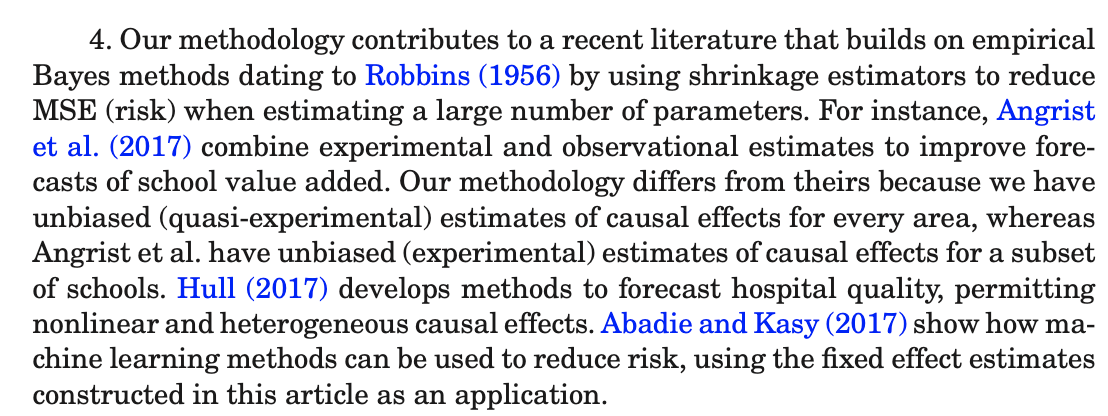
\includegraphics[scale=0.4]{figures/Chetty_n_Hendren_QJE_1.png}
  
\includegraphics[scale=0.4]{figures/Chetty_n_Hendren_QJE_2.png}
  \\
  \tiny Chetty, R., \& Hendren, N. QJE (2018). 
\end{figure}

\end{frame}

%----------------------------------------------------------------------%
\begin{frame}[fragile]
\frametitle{Empirical Bayes}

Consider the following standard Bayesian model:

\bigskip

\begin{align}
X &\sim N(\theta,1) \\
\theta &\sim N(0,\tau^2) 
\end{align}

\bigskip
\begin{itemize}
  \item Standard approach the experimenter would specify a prior value for $\tau^2$
\end{itemize}


\end{frame}
%----------------------------------------------------------------------%
\begin{frame}[fragile]
\frametitle{Empirical Bayes}
\begin{itemize}
  \item However, note that the marginal distribution of X is $N(0,\tau^2+1)$, Why?
\end{itemize}
Sketch
\begin{align}
m(X) &=\int f(X|\theta)p(\theta)d\theta \\ \nonumber
 &\propto \int exp \left(\frac{-1}{2}(x-\theta)^2\right) exp \left( \frac{-\theta^2}{2\tau^2}\right) d\theta \\ \nonumber
 &\propto \int exp \left( \frac{-1}{2} \left( (x-\theta)^2 + \frac{\theta^2}{\tau^2}\right)\right) d\theta 
\end{align}

Let's focus here $(x-\theta)^{2}+\frac{\theta^{2}}{\tau^{2}} $
\begin{align}
\approx \left(\frac{\tau^2}{\left(\tau^{2}+1\right)^2}(x)^{2}\right)+\left(\theta-\left(\frac{\tau^{2}}{\tau^{2}+1}\right)x\right)^{2} 
\end{align}

\end{frame}
%----------------------------------------------------------------------%
\begin{frame}[fragile]
\frametitle{Empirical Bayes}


then

\begin{align}
X \sim N(0,\tau^2+1)
\end{align}


\bigskip
\begin{itemize}
  \item Empirical Bayes uses this ``shortcut''.
  \item Use the data to obtain the ``unknown parameters''
\end{itemize}

\end{frame}

%----------------------------------------------------------------------%
\subsection{Robbins' Formula}
%----------------------------------------------------------------------%
\begin{frame}[fragile]
\frametitle{Robbins' Formula}
{\bf Example}: an insurance company is concerned about the claims each policy holder will make in the next year.
\begin{table}[H]
\caption{Claims data for a European automobile insurance company}
\begin{tabular}{lcccccccc}
Claims & 0    & 1    & 2   & 3  & 4  & 5 & 6 & 7 \\
\hline
Counts & 7840 & 1317 & 239 & 42 & 14 & 4 & 4 & 1 \\
\end{tabular}
\end{table}

\end{frame}
%----------------------------------------------------------------------%
\begin{frame}[fragile]
\frametitle{Robbins' Formula}

\begin{itemize}
\item It seems that we can use Bayes formula to get next years expected number of accidents
\item We suppose that $x_k$, the number of claims to be made in a single year by policy holder $k$, 
\item This follows a Poisson distribution with parameter $\theta_k$
\item Recall that the mean and variance are $\theta_k$
\end{itemize}

\begin{align}
Pr(x_k=x) = p_{\theta_k}(x)= \frac{e^{-\theta_k} \theta_k^x}{x!} \,\,\, for \,\,\, x=0,1,2,3,...
\end{align}


\end{frame}
%----------------------------------------------------------------------%
\begin{frame}[fragile]
\frametitle{Robbins' Formula}

Suppose now, that we know the prior density $g(\theta)$. Then using Bayes rule we would have

\begin{align}
E(\theta|x)&= \int_0^{\infty} \theta \pi(\theta)d\theta \\
 &=\frac{\int_0^{\infty} \theta p_{\theta_k}(x) g(\theta) d\theta }{\int_0^{\infty} p_{\theta_k}(x) g(\theta) d\theta}
\end{align}

is the expected value of $\theta$ of a customer observed to make $x$ claims in a single year. This would answer the insurance company's questions of what numbers of claims X to expect the next year from the same customer

\end{frame}
%----------------------------------------------------------------------%
\begin{frame}[fragile]
\frametitle{Robbins' Formula}
What happens if we don't know the prior? 

Note the following:

\begin{align}
E(\theta|x)&=   \frac{\int_0^{\infty} \theta[e^{-\theta} \theta^x/x!]g(\theta)d\theta}{\int_0^{\infty} [e^{-\theta} \theta^x/x!]g(\theta)d\theta}
\end{align}
\medskip

\begin{align}
E(\theta|x)&=   \frac{(x+1) \int_0^{\infty} [e^{-\theta} \theta^{x+1}/(x+1)!]g(\theta)d\theta}{\int_0^{\infty} [e^{-\theta} \theta^x/x!]g(\theta)d\theta}
\end{align}

\begin{align}
E(\theta|x)&=   \frac{(x+1) m(x+1)}{m(x)} 
\end{align}

\end{frame}


%----------------------------------------------------------------------%
\begin{frame}[fragile]
\frametitle{Robbins' Formula}
The obvious estimate of the marginal density $m(x)$ is the proportion of total counts in category $x$,
\begin{align}
\hat m(x)= \frac{y_x}{N}
\end{align}
where $N=\sum_x y_x$ 

\begin{table}[H]
\caption{Claims data for a European automobile insurance company}
\begin{tabular}{lcccccccc}
Claims & 0    & 1    & 2   & 3  & 4  & 5 & 6 & 7 \\
\hline
Counts & 7840 & 1317 & 239 & 42 & 14 & 4 & 4 & 1 \\
Mean & .168 & .363 & .527 & 1.33 & 1.43 & 46 & 1.75 & . \\
\end{tabular}
\end{table}

\end{frame}

%----------------------------------------------------------------------%
\subsection{Sabermetrics}
%----------------------------------------------------------------------%
\begin{frame}[fragile]
\frametitle{Sabermetrics: Batting Averages}

\begin{figure}[H] \centering
  \centering
  
\includegraphics[scale=0.45]{figures/simpsons-sabermetrics.jpg}
  \\
  \tiny 
\end{figure}
\end{frame}

%----------------------------------------------------------------------%
\begin{frame}[fragile]
\frametitle{Sabermetrics: Batting Averages}
\begin{itemize}
\item One of the most commonly used statistics in baseball is the batting average
\end{itemize}

\begin{align}
\text{Batting Average} = \frac{\text{number of hits (H)}}{\text{number of at-bats (AB)}}
\end{align}

\bigskip
Today we are going to explore two additional problems  and use EB:
\medskip
\begin{enumerate}
\item You want to recruit two players:  One has achieved 4 hits in 10 chances, the other 300 hits in 1000 chances.
\item Based on first few performances, can we predict what is going to be the season-long batting averages
\end{enumerate}


\end{frame}
%----------------------------------------------------------------------%
\begin{frame}[fragile]
\frametitle{Sabermetrics: Recruiting}

\begin{itemize}
  \item Let's see some data {\tiny   (Here I'm using a "clean" version of \texttt{Batting} data from the \texttt{Lahman} package)}
\end{itemize}


\tiny
\begin{Shaded}
\begin{Highlighting}[]
\tiny
\KeywordTok{require}\NormalTok{(}\StringTok{"dplyr"}\NormalTok{) }
\KeywordTok{require}\NormalTok{(}\StringTok{"tidyr"}\NormalTok{) }
\KeywordTok{require}\NormalTok{(}\StringTok{"ggplot2"}\NormalTok{) }
\end{Highlighting}
\end{Shaded}


\begin{Shaded}
\begin{Highlighting}[]
\NormalTok{career\textless{}{-}}\KeywordTok{readRDS}\NormalTok{(}\StringTok{"baseball.rds"}\NormalTok{)}
\KeywordTok{head}\NormalTok{(career)}
\end{Highlighting}
\end{Shaded}

\begin{small}
\begin{verbatim}
## # A tibble: 6 x 4
##   name               H    AB average
##   <chr>          <int> <int>   <dbl>
## 1 Hank Aaron      3771 12364  0.305 
## 2 Tommie Aaron     216   944  0.229 
## 3 Andy Abad          2    21  0.0952
## 4 John Abadie       11    49  0.224 
## 5 Ed Abbaticchio   772  3044  0.254 
## 6 Fred Abbott      107   513  0.209
\end{verbatim}
\end{small}

\end{frame}

%----------------------------------------------------------------------%
\begin{frame}[fragile]
\frametitle{Batting Averages}

\begin{itemize}
  \item Best Batting Averages?
\end{itemize} 

\begin{small}
\begin{verbatim}
## # A tibble: 6 x 4
##   name             H    AB average
##   <chr>        <int> <int>   <dbl>
## 1 Roe Skidmore     1     1       1
## 2 Charlie Snow     1     1       1
## 3 Matt Tupman      1     1       1
## 4 Allie Watt       1     1       1
## 5 Al Wright        1     1       1
## 6 George Yantz     1     1       1
\end{verbatim}
\end{small}

\end{frame}

%----------------------------------------------------------------------%
\begin{frame}[fragile]
\frametitle{Batting Averages}


\begin{itemize}
  \item Worst Batting Averages?
\end{itemize}

\begin{small}
\begin{verbatim}
## # A tibble: 6 x 4
##   name                  H    AB average
##   <chr>             <int> <int>   <dbl>
## 1 Frank Abercrombie     0     4       0
## 2 Horace Allen          0     7       0
## 3 Pete Allen            0     4       0
## 4 Walter Alston         0     1       0
## 5 Bill Andrus           0     9       0
## 6 Wyman Andrus          0     4       0
\end{verbatim}
\end{small}


\end{frame}

%----------------------------------------------------------------------%
\begin{frame}[fragile]
\frametitle{Sabermetrics: Recruiting}
\begin{itemize}
\item You want a ``true'' measure of batting performance
\medskip
\item We know by history that most batting averages are between .210 and .360 
\medskip
\item  We can model




\begin{align}
\text{Batting Average} \sim Binomial(N,\theta)
\end{align}


\item where $N$ is the times at bat and $\theta$ is the proportion of successes
\end{itemize}

\end{frame}

%----------------------------------------------------------------------%
\begin{frame}[fragile]
\frametitle{Sabermetrics: Recruiting}

\begin{itemize}

\item We can incorporate historical data with a prior 
\medskip
\item We use a conjugate prior for simplicity. 
\end{itemize}



\begin{align}
p(\theta) \sim Beta(\alpha_0,\beta_0)
\end{align}

The posterior is:
\begin{align}
\pi(\theta)\sim Beta(\alpha_0+hits,\beta_0+N-hits)
\end{align}

\medskip
\begin{itemize}
  \item We don't know $\alpha_0$ and $\beta_0$. We could use the fact that most batting averages are between .210 and .360. Select $\alpha_0$ and $\beta_0$ accordingly.
  \medskip
  \item Or we can use Empirical Bayes: estimate these parameters from the data.
\end{itemize}


\end{frame}
%----------------------------------------------------------------------%
\begin{frame}[fragile]
\frametitle{Batting Averages}
Histogram of batting averages

\bigskip
\bigskip
\begin{figure}[H] \centering
  \centering
  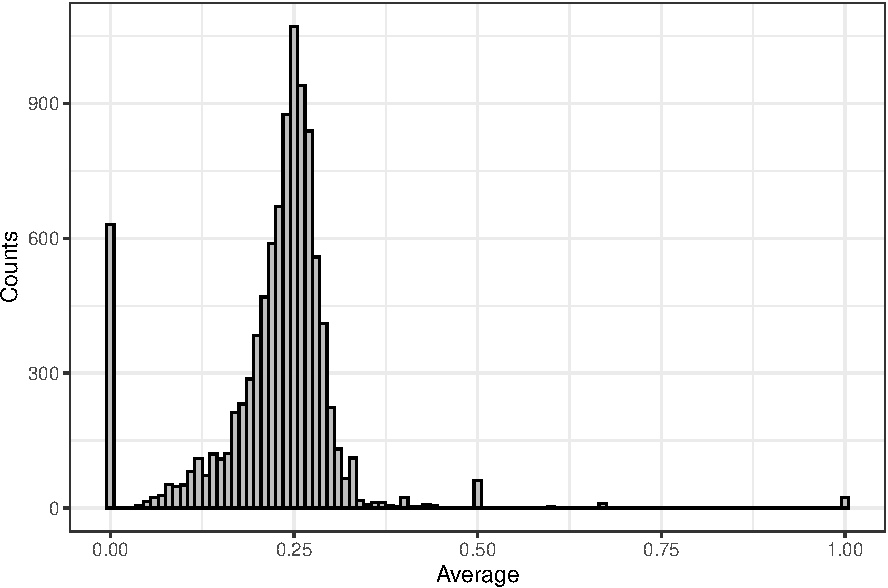
\includegraphics[scale=0.6]{figures/average_hist.pdf}
  \\
  \tiny 
\end{figure}



\end{frame}


%----------------------------------------------------------------------%
\begin{frame}[fragile]
\frametitle{Batting Averages}
Restrict our sample to those data points that are  informative (individuals that have gone at bat at least 500 times)

\bigskip

\begin{figure}[H] \centering
  \centering
  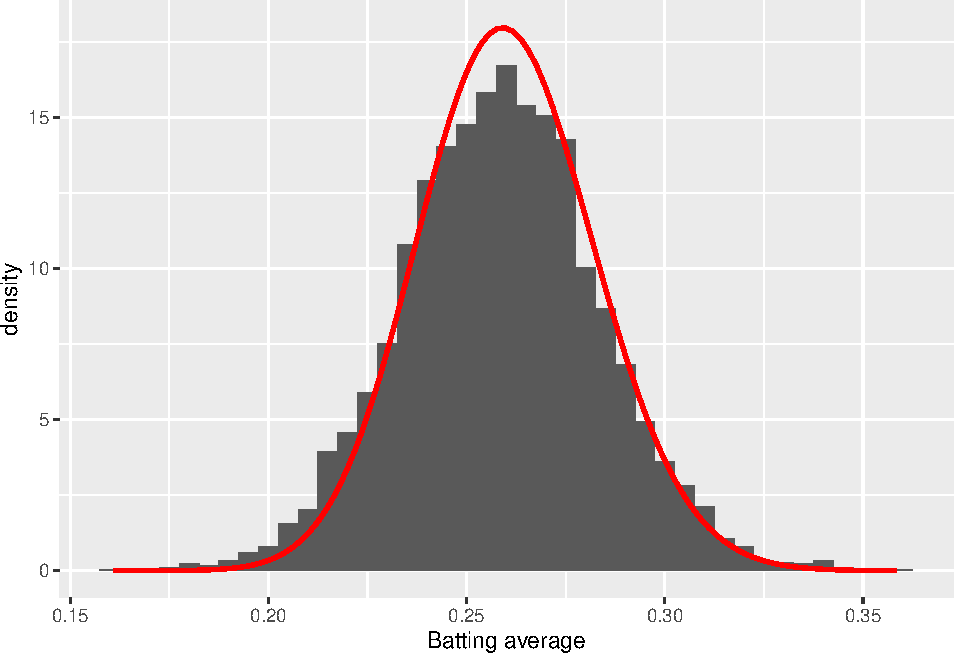
\includegraphics[scale=0.4]{figures/av_hist_w_mle.pdf}
  \\
  \tiny 
\end{figure}


\end{frame}

\begin{frame}[fragile]
\frametitle{Batting Averages}
How we find the parameters that find the red line $\rightarrow$ MLE! We know that

\begin{align}
f(x_i|\alpha_0,\beta_0)=\frac{\Gamma(\alpha_0+\beta_0)}{\Gamma(\alpha_0)\Gamma(\beta_0)}x_i^{\alpha_0-1}\left(1-x_i\right)^{\beta_0-1}
\end{align}

The log likelihood 
\begin{footnotesize}
\begin{align}
l(\alpha_0,\beta_0|X) = n . log(\frac{\Gamma(\alpha_0+\beta_0)}{\Gamma(\alpha_0)\Gamma(\beta_0)}) + \sum_{i=1}^n ((\alpha_0-1)log(x_i)+(\beta_0-1)log(1-x_i))
\end{align}
\end{footnotesize}


In \texttt{R}
\footnotesize
\begin{Shaded}
\begin{Highlighting}[]
\CommentTok{\# log{-}likelihood function}
\NormalTok{ll \textless{}{-}}\StringTok{ }\ControlFlowTok{function}\NormalTok{(alpha, beta) \{}
\OperatorTok{{-}}\KeywordTok{sum}\NormalTok{(VGAM}\OperatorTok{::}\KeywordTok{dbetabinom.ab}\NormalTok{(x, total, alpha, beta, }\DataTypeTok{log =} \OtherTok{TRUE}\NormalTok{))}
\NormalTok{\}}
\CommentTok{\# maximum likelihood estimation}
\NormalTok{m \textless{}{-}}\StringTok{ }\KeywordTok{mle}\NormalTok{(ll, }\DataTypeTok{start =} \KeywordTok{list}\NormalTok{(}\DataTypeTok{alpha =} \DecValTok{1}\NormalTok{, }\DataTypeTok{beta =} \DecValTok{10}\NormalTok{), }
\DataTypeTok{method =} \StringTok{"L{-}BFGS{-}B"}\NormalTok{, }\DataTypeTok{lower =} \KeywordTok{c}\NormalTok{(}\FloatTok{0.0001}\NormalTok{, }\FloatTok{.1}\NormalTok{))}
\NormalTok{ab \textless{}{-}}\StringTok{ }\KeywordTok{coef}\NormalTok{(m) }
\end{Highlighting}
\end{Shaded}


\end{frame}
%----------------------------------------------------------------------%
\begin{frame}[fragile]
\frametitle{Batting Averages}
\footnotesize
\begin{Shaded}
\begin{Highlighting}[]
\NormalTok{alpha0 \textless{}{-}}\StringTok{ }\NormalTok{ab[}\DecValTok{1}\NormalTok{]}
101.7319 
\NormalTok{beta0 \textless{}{-}}\StringTok{ }\NormalTok{ab[}\DecValTok{2}\NormalTok{]}
289.046 
\end{Highlighting}
\end{Shaded}



\begin{figure}[H] \centering
  \centering
  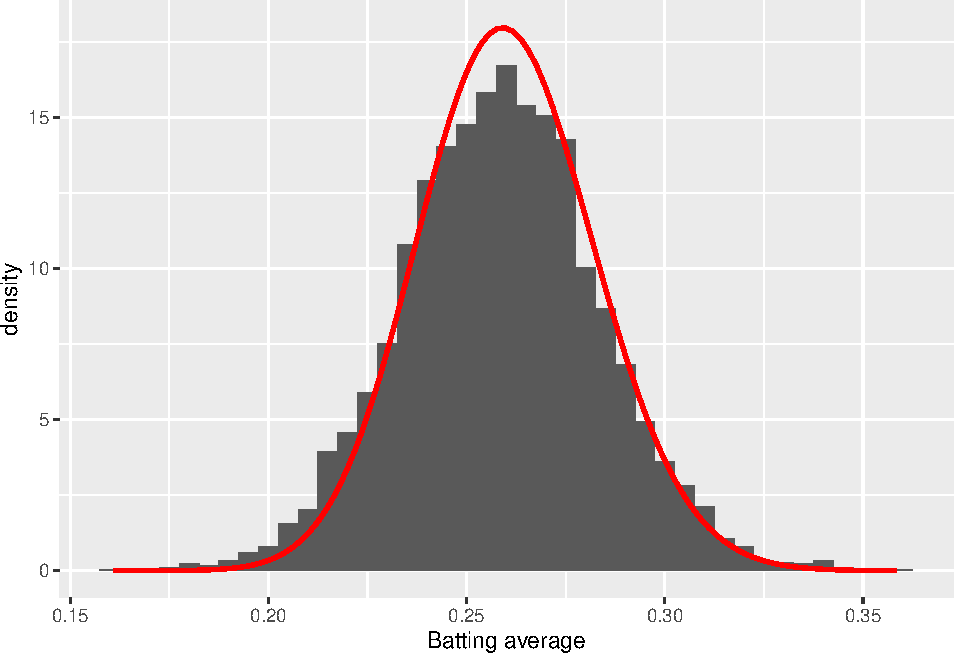
\includegraphics[scale=0.4]{figures/av_hist_w_mle.pdf}
  \\
  \tiny 
\end{figure}


\end{frame}
%----------------------------------------------------------------------%
\begin{frame}[fragile]
\frametitle{Batting Averages}

We can use the estimated average based on the posterior mean

\begin{align}
E(\theta|X)=\frac{\alpha_0+hits}{\alpha_0+\beta_0+N}
\end{align}


\begin{itemize}
  \item Now we can ask again: who are the best batters by this improved estimate?
\end{itemize}



\end{frame}
%----------------------------------------------------------------------%
\begin{frame}[fragile]
\frametitle{Sabermetrics: Recruiting}

\begin{itemize}
  \item Now we can ask again: who are the best batters by this improved estimate?
\end{itemize}


\begin{footnotesize}
\begin{verbatim}
## # A tibble: 5 x 5
##   name                     H    AB average eb_estimate
##   <chr>                <int> <int>   <dbl>       <dbl>
## 1 Rogers Hornsby        2930  8173   0.358       0.354
## 2 Shoeless Joe Jackson  1772  4981   0.356       0.349
## 3 Ed Delahanty          2597  7510   0.346       0.342
## 4 Billy Hamilton        2164  6283   0.344       0.339
## 5 Willie Keeler         2932  8591   0.341       0.338
\end{verbatim}
\end{footnotesize}

\begin{itemize}
\item Who are the \emph{worst} batters?
\end{itemize}
\begin{footnotesize}
\begin{verbatim}
## # A tibble: 5 x 5
##   name                H    AB average eb_estimate
##   <chr>           <int> <int>   <dbl>       <dbl>
## 1 Bill Bergen       516  3028   0.170       0.181
## 2 Ray Oyler         221  1265   0.175       0.195
## 3 Henry Easterday   203  1129   0.180       0.201
## 4 John Vukovich      90   559   0.161       0.202
## 5 George Baker       74   474   0.156       0.203
\end{verbatim}
\end{footnotesize}

\end{frame}
%----------------------------------------------------------------------%
\begin{frame}[fragile]
\frametitle{Sabermetrics: Recruiting}

We can see how EB changed all of the batting average estimates:

\begin{figure}[H] \centering
  \centering
  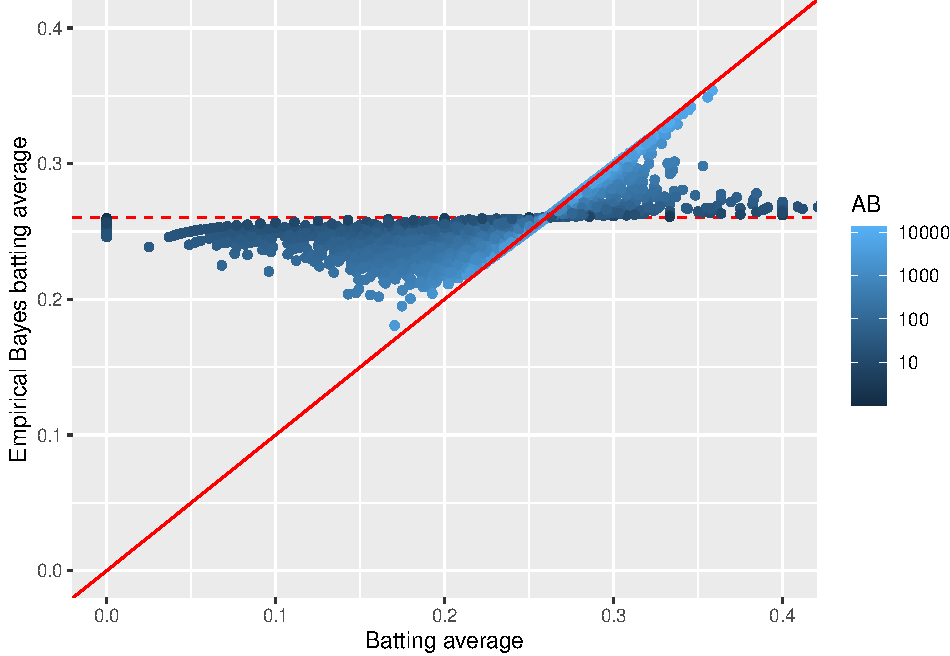
\includegraphics[scale=0.5]{figures/shrinkage_averages}
  \\
  \tiny 
\end{figure}



\end{frame}
%----------------------------------------------------------------------%
\begin{frame}[fragile]
\frametitle{Sabermetrics: Predicting Batting Averages}

\begin{itemize}
\item Now supposed you want to know the end of season final batting average of players, after observing them their 45 first times at bat.
\end{itemize}


\begin{table}[H]
\begin{tabular}{lcc}
\hline
\hline
Player & Observed & Final \\
\hline
1 & 0.395 & 0.346 \\
2 & 0.355 & 0.279 \\
3 & 0.313 & 0.276 \\
4 & 0.291 & 0.266 \\
5 & 0.247 & 0.271 \\
6 & 0.224 & 0.266 \\
7 & 0.175 & 0.318 \\
\hline
\hline
\end{tabular}
\end{table}
\end{frame}
%----------------------------------------------------------------------%
\begin{frame}[fragile]
\frametitle{Sabermetrics: Predicting Batting Averages}

\begin{itemize}
\item Recall that we can think each time at bat can be thought as a binomial trial, with $\theta$ the probability of success equal to the player's true batting average.
\item With 45 trials, we can ``reasonably'' use a Normal Approximation.
\end{itemize}

\begin{align}
  X_i \sim N(\theta_i,\sigma^2)
\end{align}
where

\begin{itemize}
  \item $\theta_i$ is the true batting average for player $i$
  \item $\sigma^2$ is the known variance that equals $(0.0659)^2$
\end{itemize}
We are going to use also a normal prior

\begin{align}
  \theta_i \sim N(\mu,\tau^2)
\end{align}

\end{frame}
%----------------------------------------------------------------------%
\begin{frame}[fragile]
\frametitle{Sabermetrics: Predicting Batting Averages}
With this model the posterior mean for $\theta_i$ is $E(\theta_i|X_i)$

\begin{align}
E(\theta_i|X_i)=\frac{\sigma^2}{\sigma^2+\tau^2}\mu + \frac{\tau^2}{\sigma^2+\tau^2} X_i
\end{align}
Note that the marginal of $X_i$

\begin{align}
m(X_i)\sim N(\mu,\sigma^2+\tau^2)\,\,\,i=1,\dots,n
\end{align}

with these we can construct estimates of $E(\theta_i|X_i)$, note that

\begin{align}
E(\bar X)&=\mu \\
E\left[ \frac{(n-3)\sigma^2}{\sum(X_i-\bar X)^2}\right]&=\frac{\sigma^2}{\sigma^2+\tau^2}
\end{align}



\end{frame}
%----------------------------------------------------------------------%
\begin{frame}[fragile]
\frametitle{Sabermetrics: Predicting Batting Averages}

The empirical Bayes estimator of $\theta_i$ is then
\begin{footnotesize}
  \begin{align}
    \delta(X_i)= \left[ \frac{(n-3)\sigma^2}{\sum(X_i-\bar X)^2}\right] \bar X + \left[ 1- \frac{(n-3)\sigma^2}{\sum(X_i-\bar X)^2}\right] X_i
  \end{align}
\end{footnotesize}


\begin{table}[]
\begin{tabular}{lcccc}
\hline
\hline
Player & Observed & Final & Empirical Bayes  \\
\hline
1      & 0.395    & 0.346 & 0.341            \\
2      & 0.355    & 0.279 & 0.321            \\
3      & 0.313    & 0.276 & 0.299            \\
4      & 0.291    & 0.266 & 0.288            \\
5      & 0.247    & 0.271 & 0.266            \\
6      & 0.224    & 0.266 & 0.255            \\
7      & 0.175    & 0.318 & 0.230           \\
\hline
\hline
\end{tabular}
\end{table}

\begin{itemize}
\item RMSE Observed 6.861903
\item RMSE EB 3.918203
\end{itemize}
\end{frame}
%----------------------------------------------------------------------%
\begin{frame}[fragile]
\frametitle{Sabermetrics: Predicting Batting Averages}

\begin{figure}[H] \centering
  \centering
  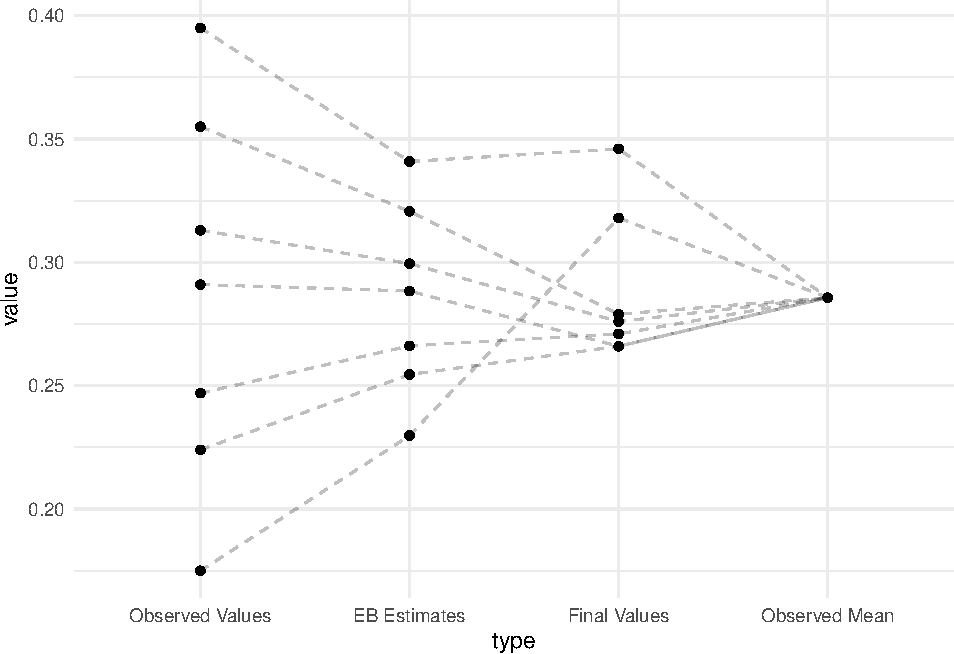
\includegraphics[scale=0.5]{figures/shrinkage_future}
  \\
  \tiny 
\end{figure}



\end{frame}
%----------------------------------------------------------------------%
\begin{frame}
\frametitle{Review \& Next Steps}
  
  \begin{itemize} 
    \item Recap Bayesian
    \medskip
    \item Empirical Bayes Examples
    
  \bigskip  

  \item  {\bf Next Week: Spatial Econometrics} 
  \bigskip
  \item  {\bf Next Week:} Problem set 2. 
  \bigskip
  
  
  
  \end{itemize}


\end{frame}


%----------------------------------------------------------------------%

\section{Further Readings}
%----------------------------------------------------------------------%
\begin{frame}
\frametitle{Further Readings}
\footnotesize
\begin{itemize}
  \item Casella, G., \& Berger, R. L. (2002). Statistical inference (Vol. 2, pp. 337-472). Pacific Grove, CA: Duxbury. Chapter 7
  \medskip
  \item Casella, G. (1985). An introduction to empirical Bayes data analysis. The American Statistician, 39(2), 83-87.
  \medskip
   \item Chetty, R., \& Hendren, N. (2018). The impacts of neighborhoods on intergenerational mobility II: County-level estimates. The Quarterly Journal of Economics, 133(3), 1163-1228.
  \medskip
  \item Efron, B., \& Hastie, T. (2016). Computer age statistical inference (Vol. 5). Cambridge University Press. Chapter 6
  \medskip
  \item Robinson, D. (2017). Introduction to Empirical Bayes: Examples from Baseball Statistics. 2017.
  \medskip
  \item Gu, J., \& Koenker, R. (2017). Empirical Bayesball remixed: Empirical Bayes methods for longitudinal data. Journal of Applied Econometrics, 32(3), 575-599.
  
\end{itemize}

\end{frame}

%----------------------------------------------------------------------%

\end{document}

%----------------------------------------------------------------------%
%----------------------------------------------------------------------%

